\documentclass[aps,reprint,superscriptaddress,10pt]{revtex4-2}
\usepackage{kotex}
\usepackage[HWP]{dhucs-interword}
\usepackage[dvips]{color}
\usepackage{graphicx}
\usepackage{bm}
\usepackage{amsmath}
\usepackage{tikz}
\usepackage{mhchem}
\usepackage{booktabs}
\usepackage{multirow}
\usepackage{array}
\usepackage{tikz}

\begin{document}
\title{응집물질물리실험 결과보고서 \\
\small 실험주제 : Photo lithography}

\author{HuiJae-Lee}\email{hjlee6674@inha.edu}
\affiliation{Physics Department, Inha University}

\date{\today}


\begin{abstract}

 \end{abstract}
 
 \maketitle
 
\section{Process}
\begin{itemize}
  \item[1. ]
  유리 기판의 표면을 아세톤과 에탄올로 깨끗하게 세척한다.
  \item[2. ]
  유리 기판의 표면에 감광물질을 도포한다(FIG.~\ref{fig:photoresist}). 
  
  \begin{figure}[htbp]
    \centering
    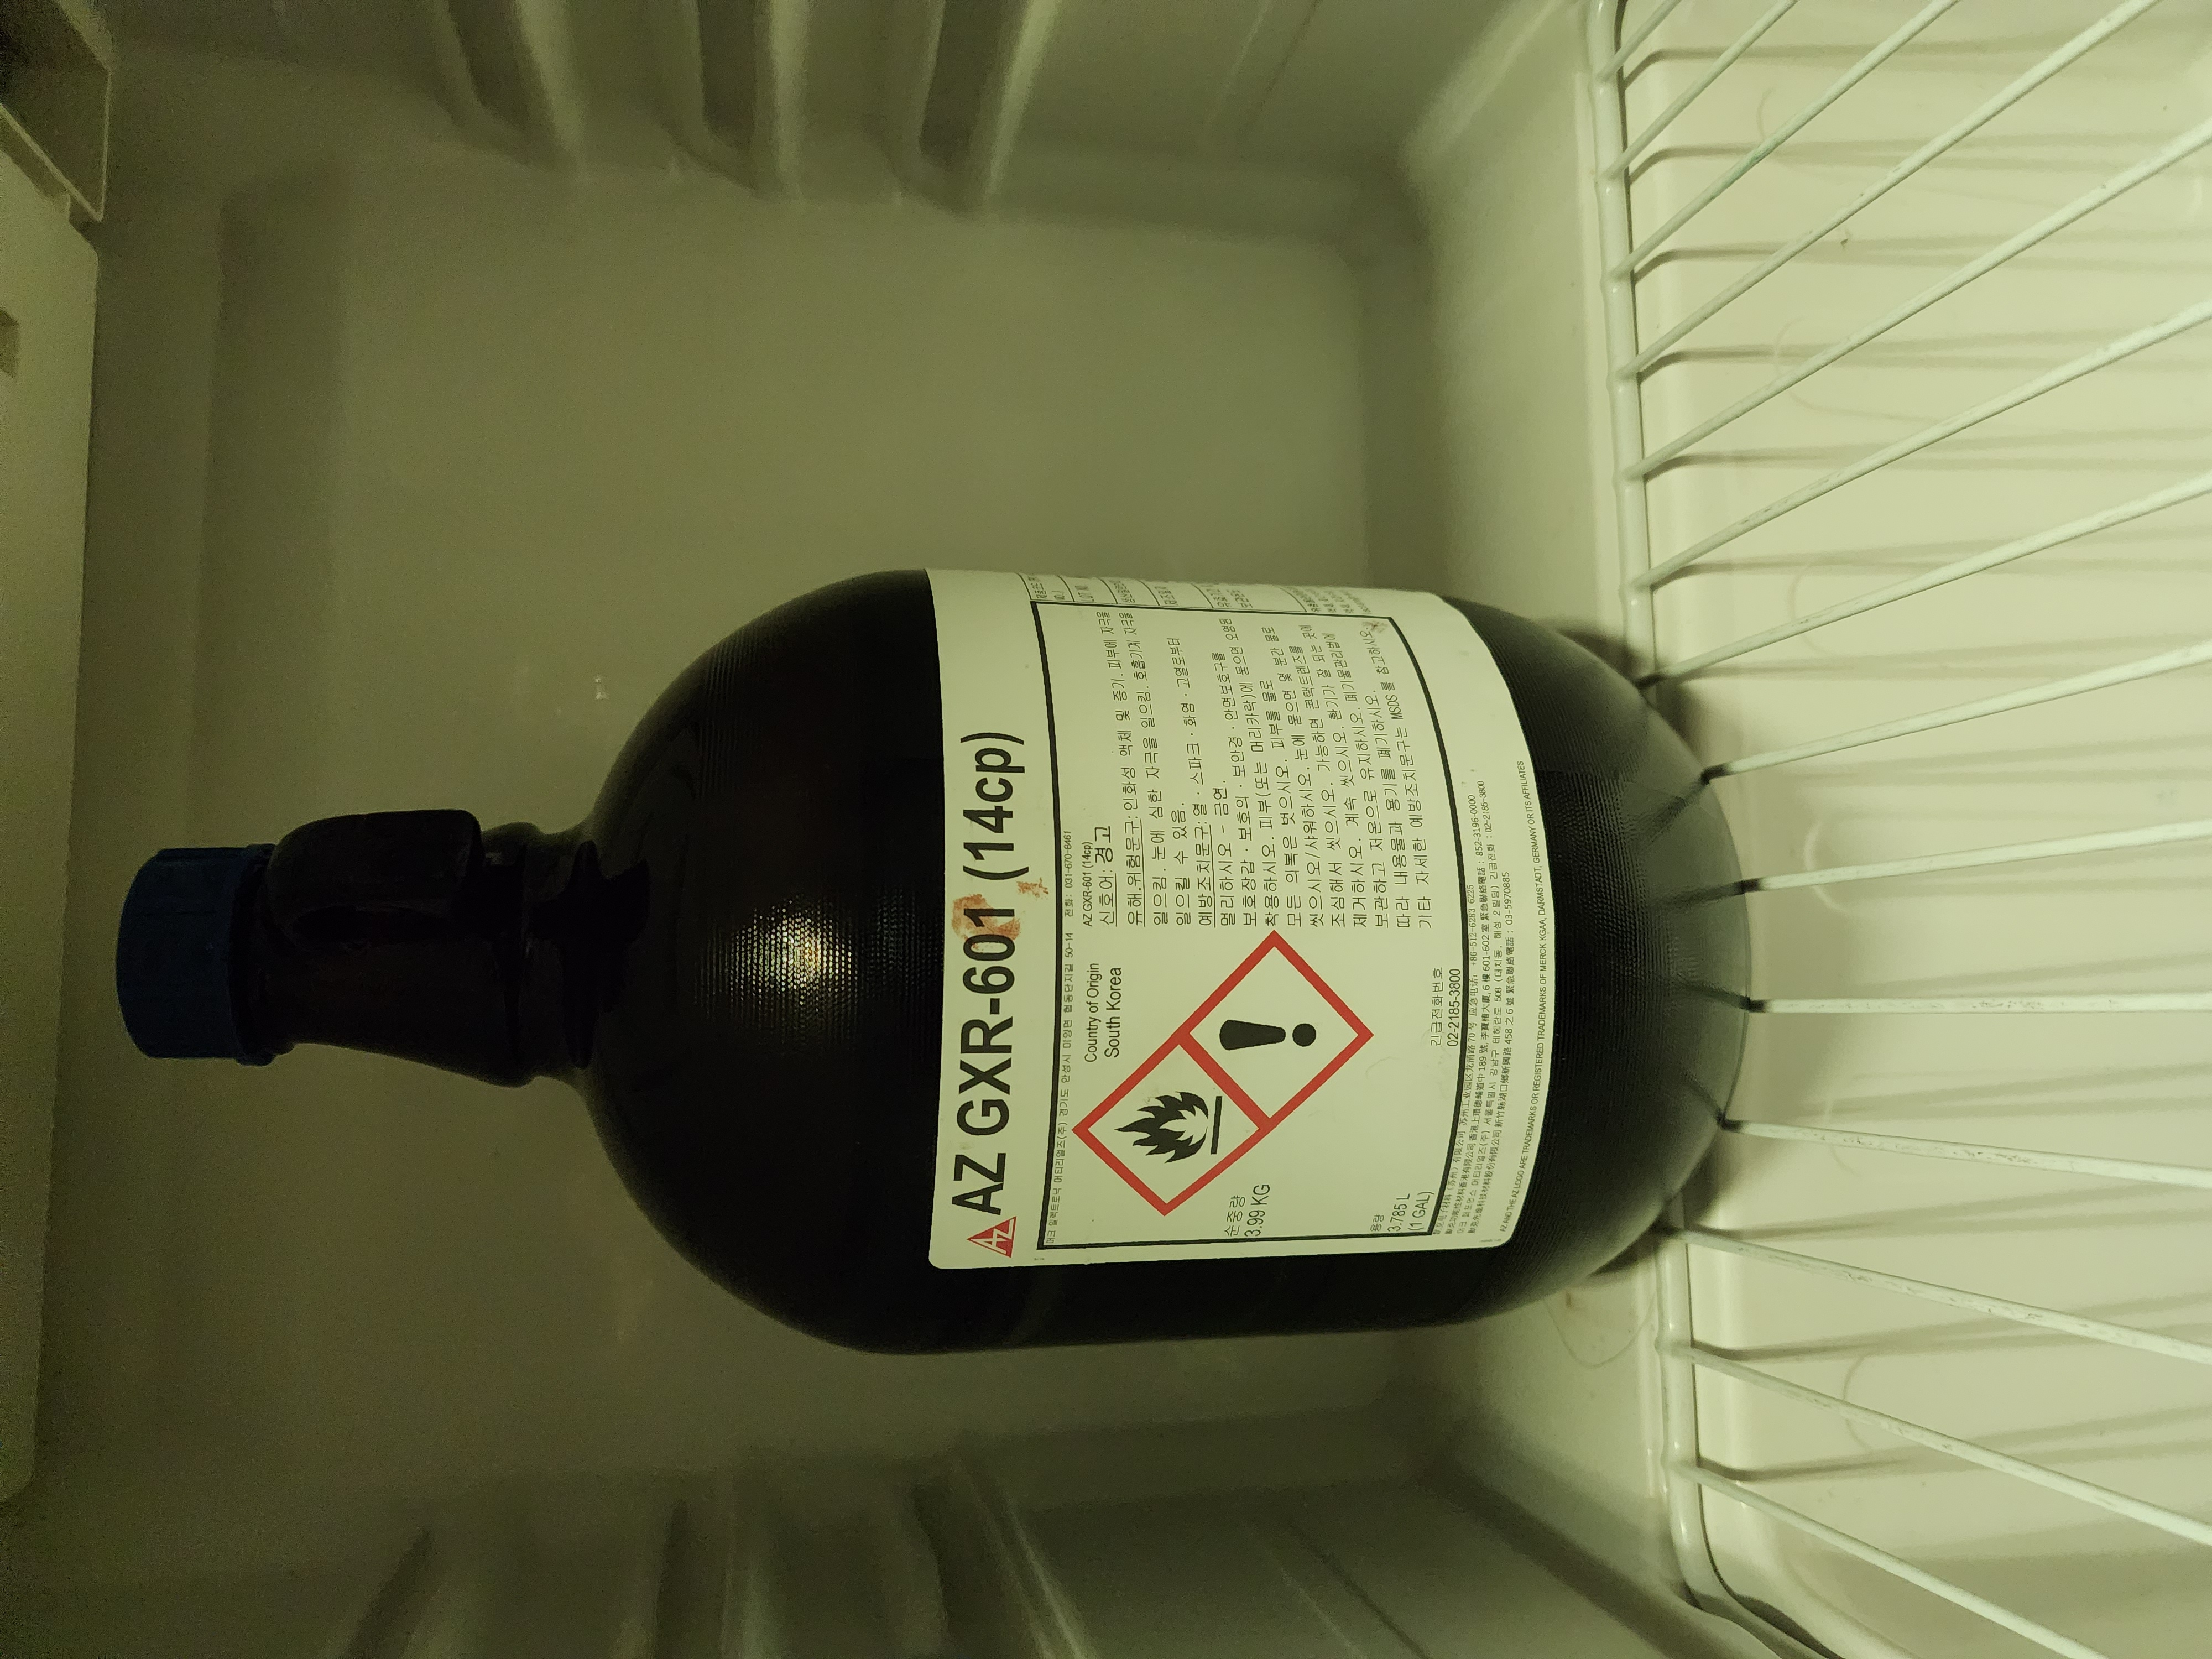
\includegraphics[scale=0.04,angle=270]{photoresist.JPG}
    \caption{감광물질 도포에 사용한 감광물질 AZ GXR-601(14cp).}
    \label{fig:photoresist}
  \end{figure}
  
  
  감광물질 토포에는 스핀 코터를 사용하며
  네개의 기판을 각각 1000 RPM, 2000 RPM, 3000 RPM, 4000 RPM의 속도로 회전시켜
  감광물질이 표면에 잘 펴지도록 한다. 기기가 설정한 속도까지 도달하는데 10초,
  설정한 속도를 유지하는데 10초, 설정한 속도로부터 멈추는데 10초가 
  소모되도록 세팅하였다(FIG.~\ref{fig:spin}).
  \begin{figure}[htbp]
    \centering
    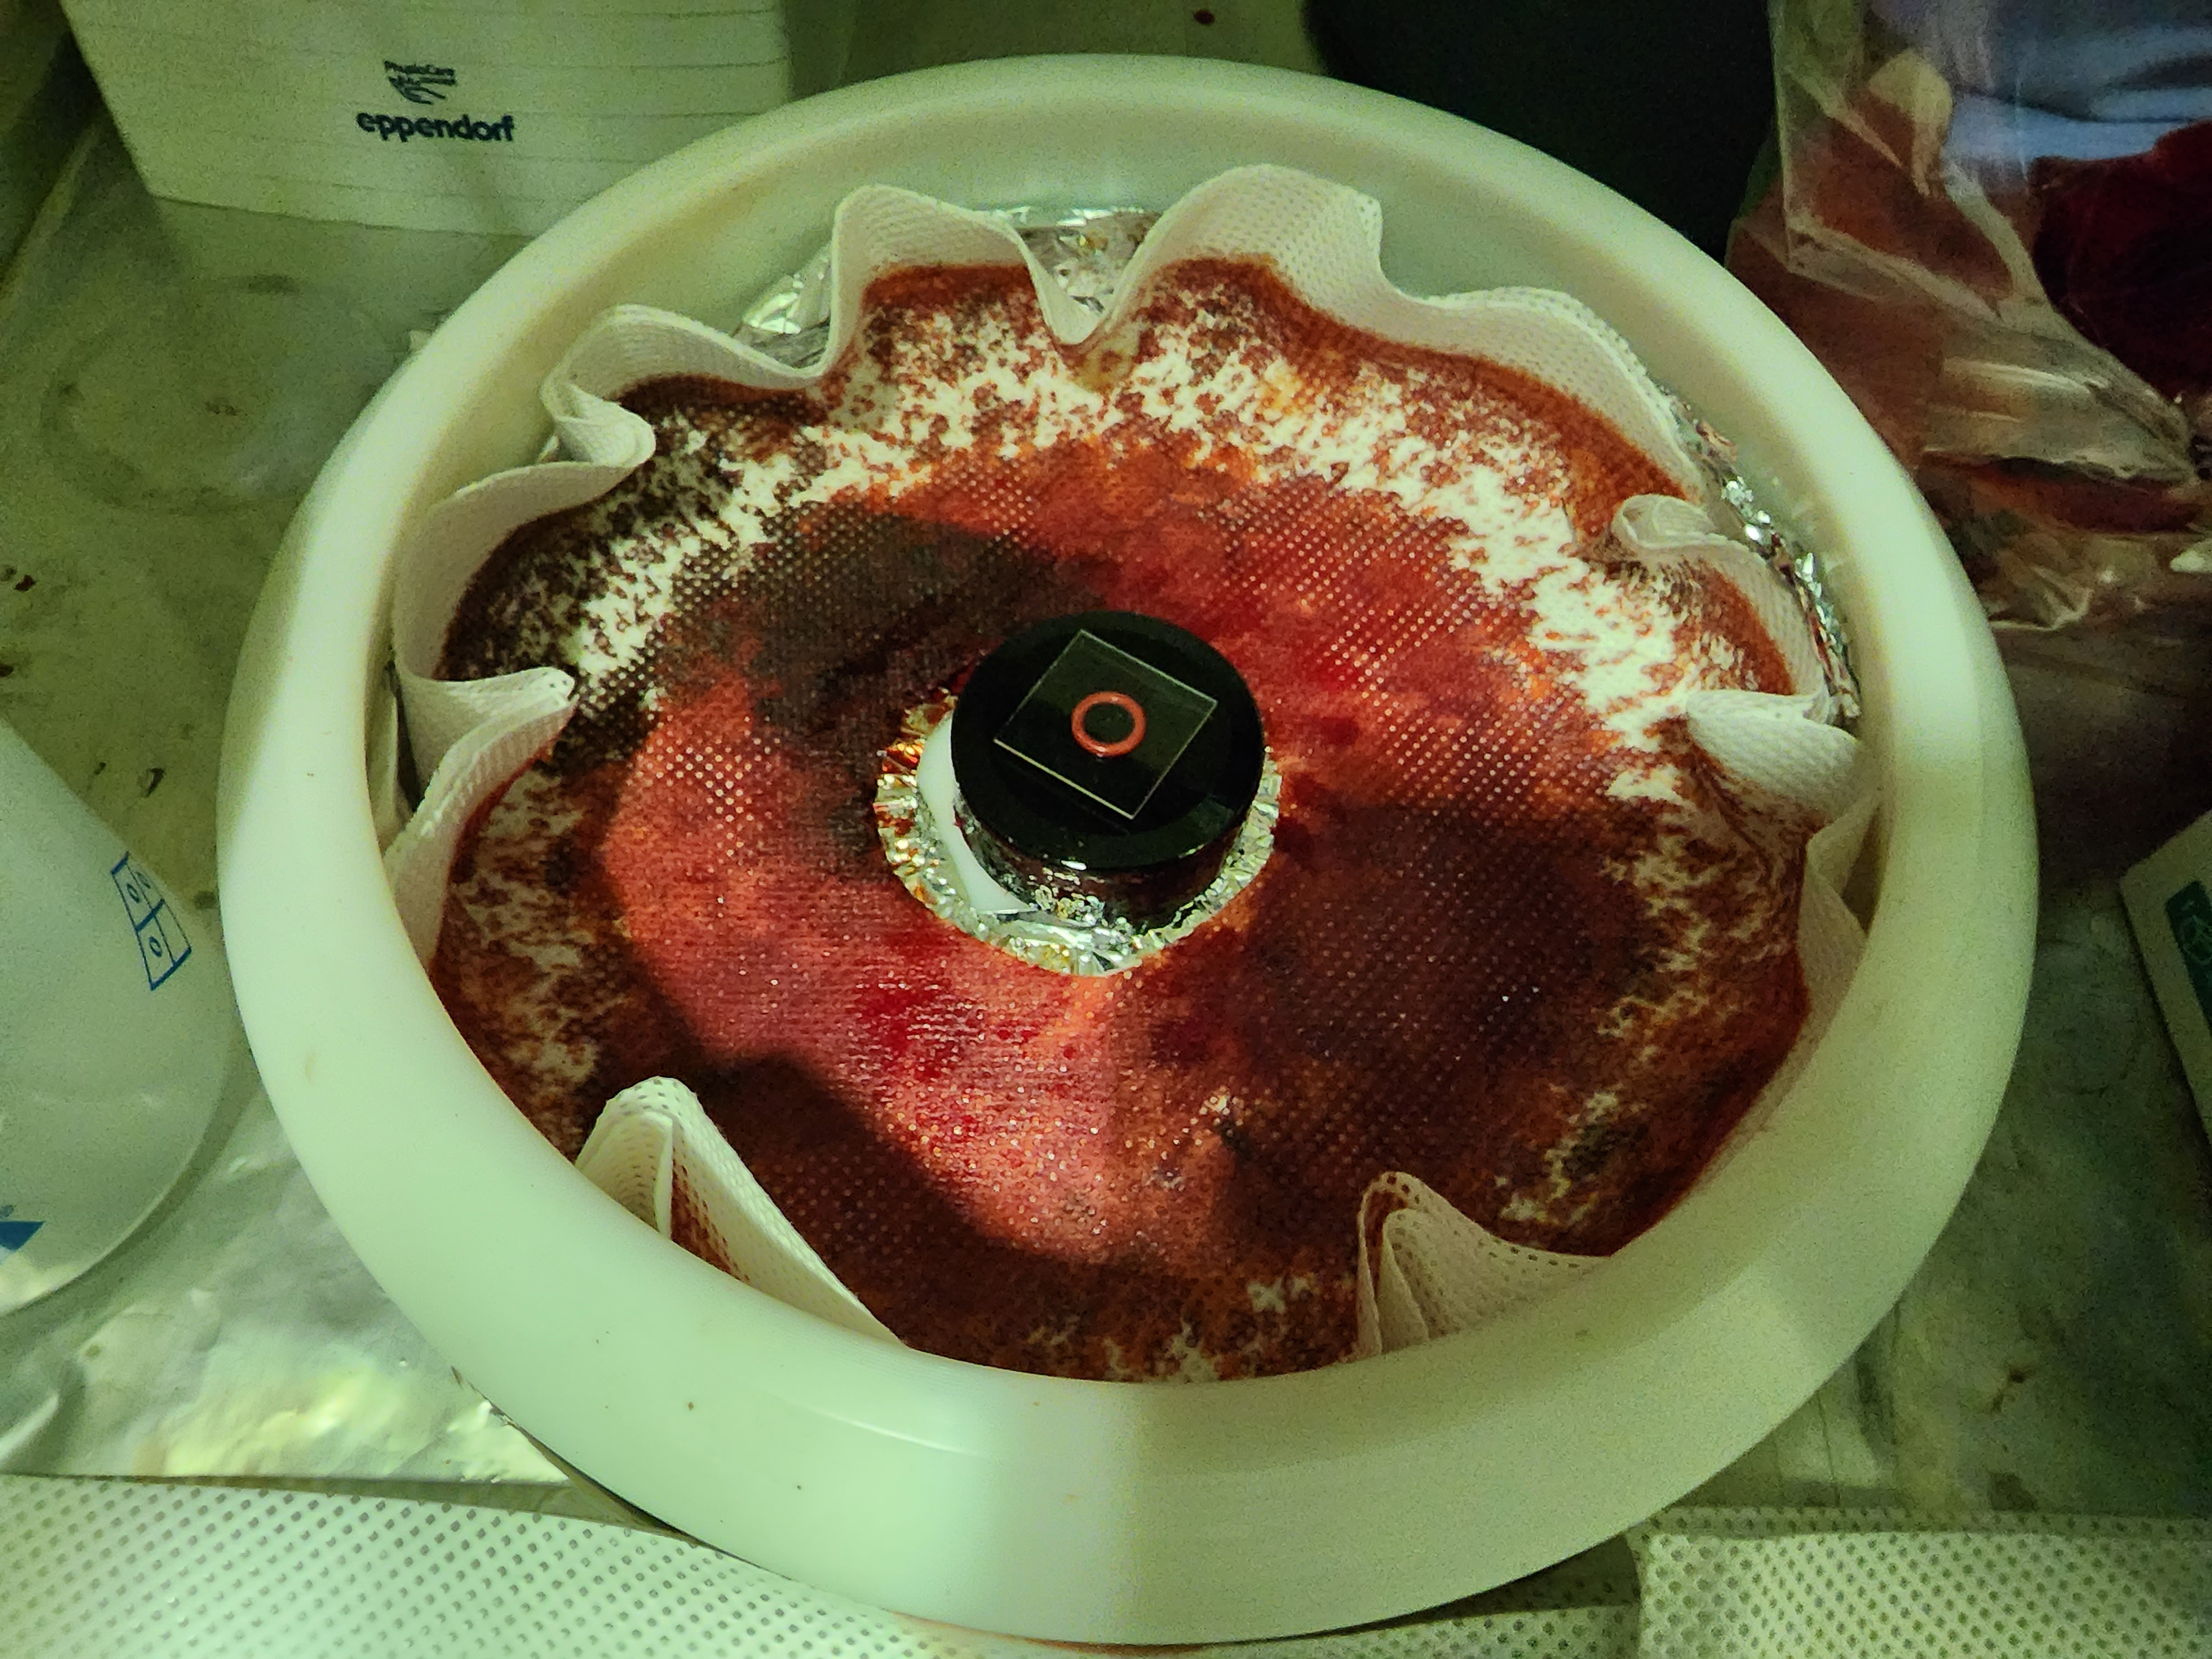
\includegraphics[scale=0.04]{spin.JPG}
    \caption{감광물질 도포에 사용한 스핀 코터. 가운데 빨간 원 위에 기판을 올리면
    기기가 진공을 만들어 기판을 고정시킨다.}
    \label{fig:spin}
  \end{figure}

  \begin{itemize}
    \item[a. ] 기판을 스핀 코터 위에 올려 고정하고 스포이드를 이용해 감광물질이
    표면 전체를 덮도록 뿌려준다.
    \item[b. ] 기기의 뚜껑을 닫고 도포를 진행한다.
    \item[c. ] 도포가 끝난 기판은 바로 soft baking 단계를 진행한다.
    \item[d. ] a ~ c의 과정을 모든 기판에 대해 반복하여 진행한다. 
  \end{itemize}
  \item[3. ]
  도포가 끝난 기판을 가열하여 감광물질이 표면에 더 잘 흡착되도록 한다.
  각 기판을 90~$^\circ$C의 온도에 90초 간 가열하였다(FIG.~\ref{fig:bake}).
  \begin{figure}[htbp]
    \centering
    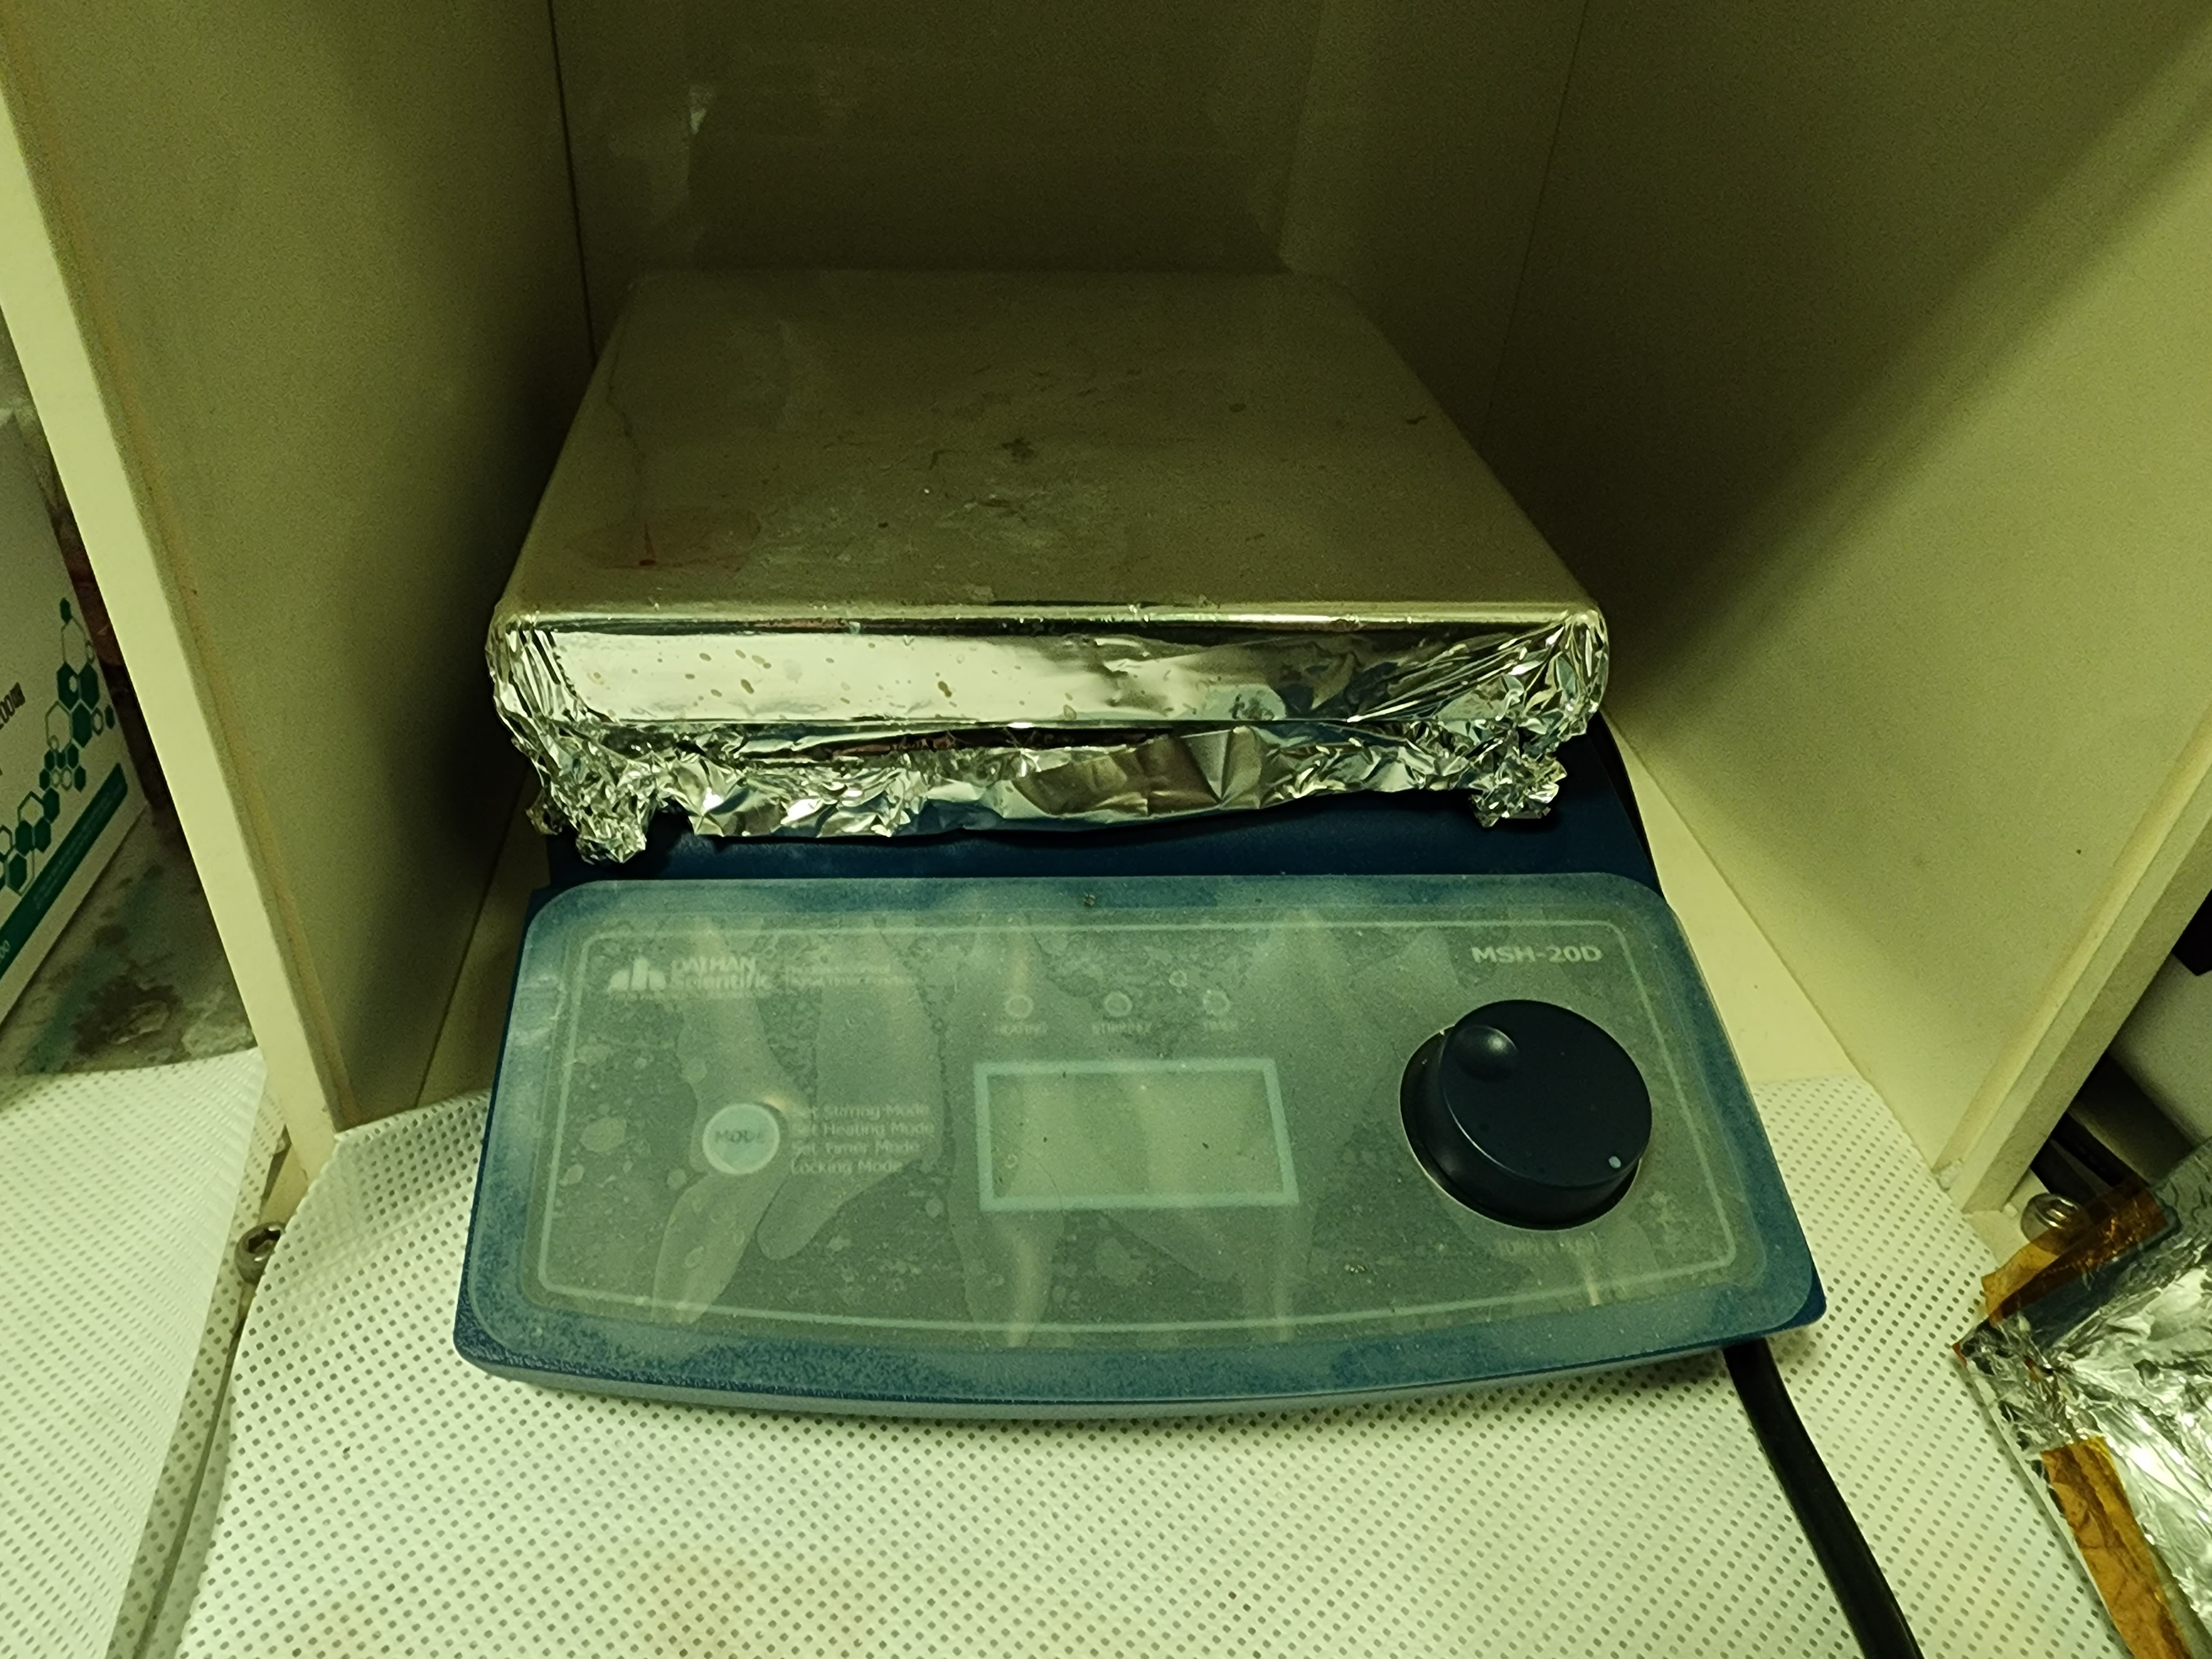
\includegraphics[scale=0.04]{bake.JPG}
    \caption{Soft baking, hard baking에 사용한 핫플레이트.}
    \label{fig:bake}
  \end{figure}

  \item[4. ] 각 기판에 자외선을 조사한다(FIG.~\ref{fig:violet}). 

  \begin{figure}[htbp]
    \centering
    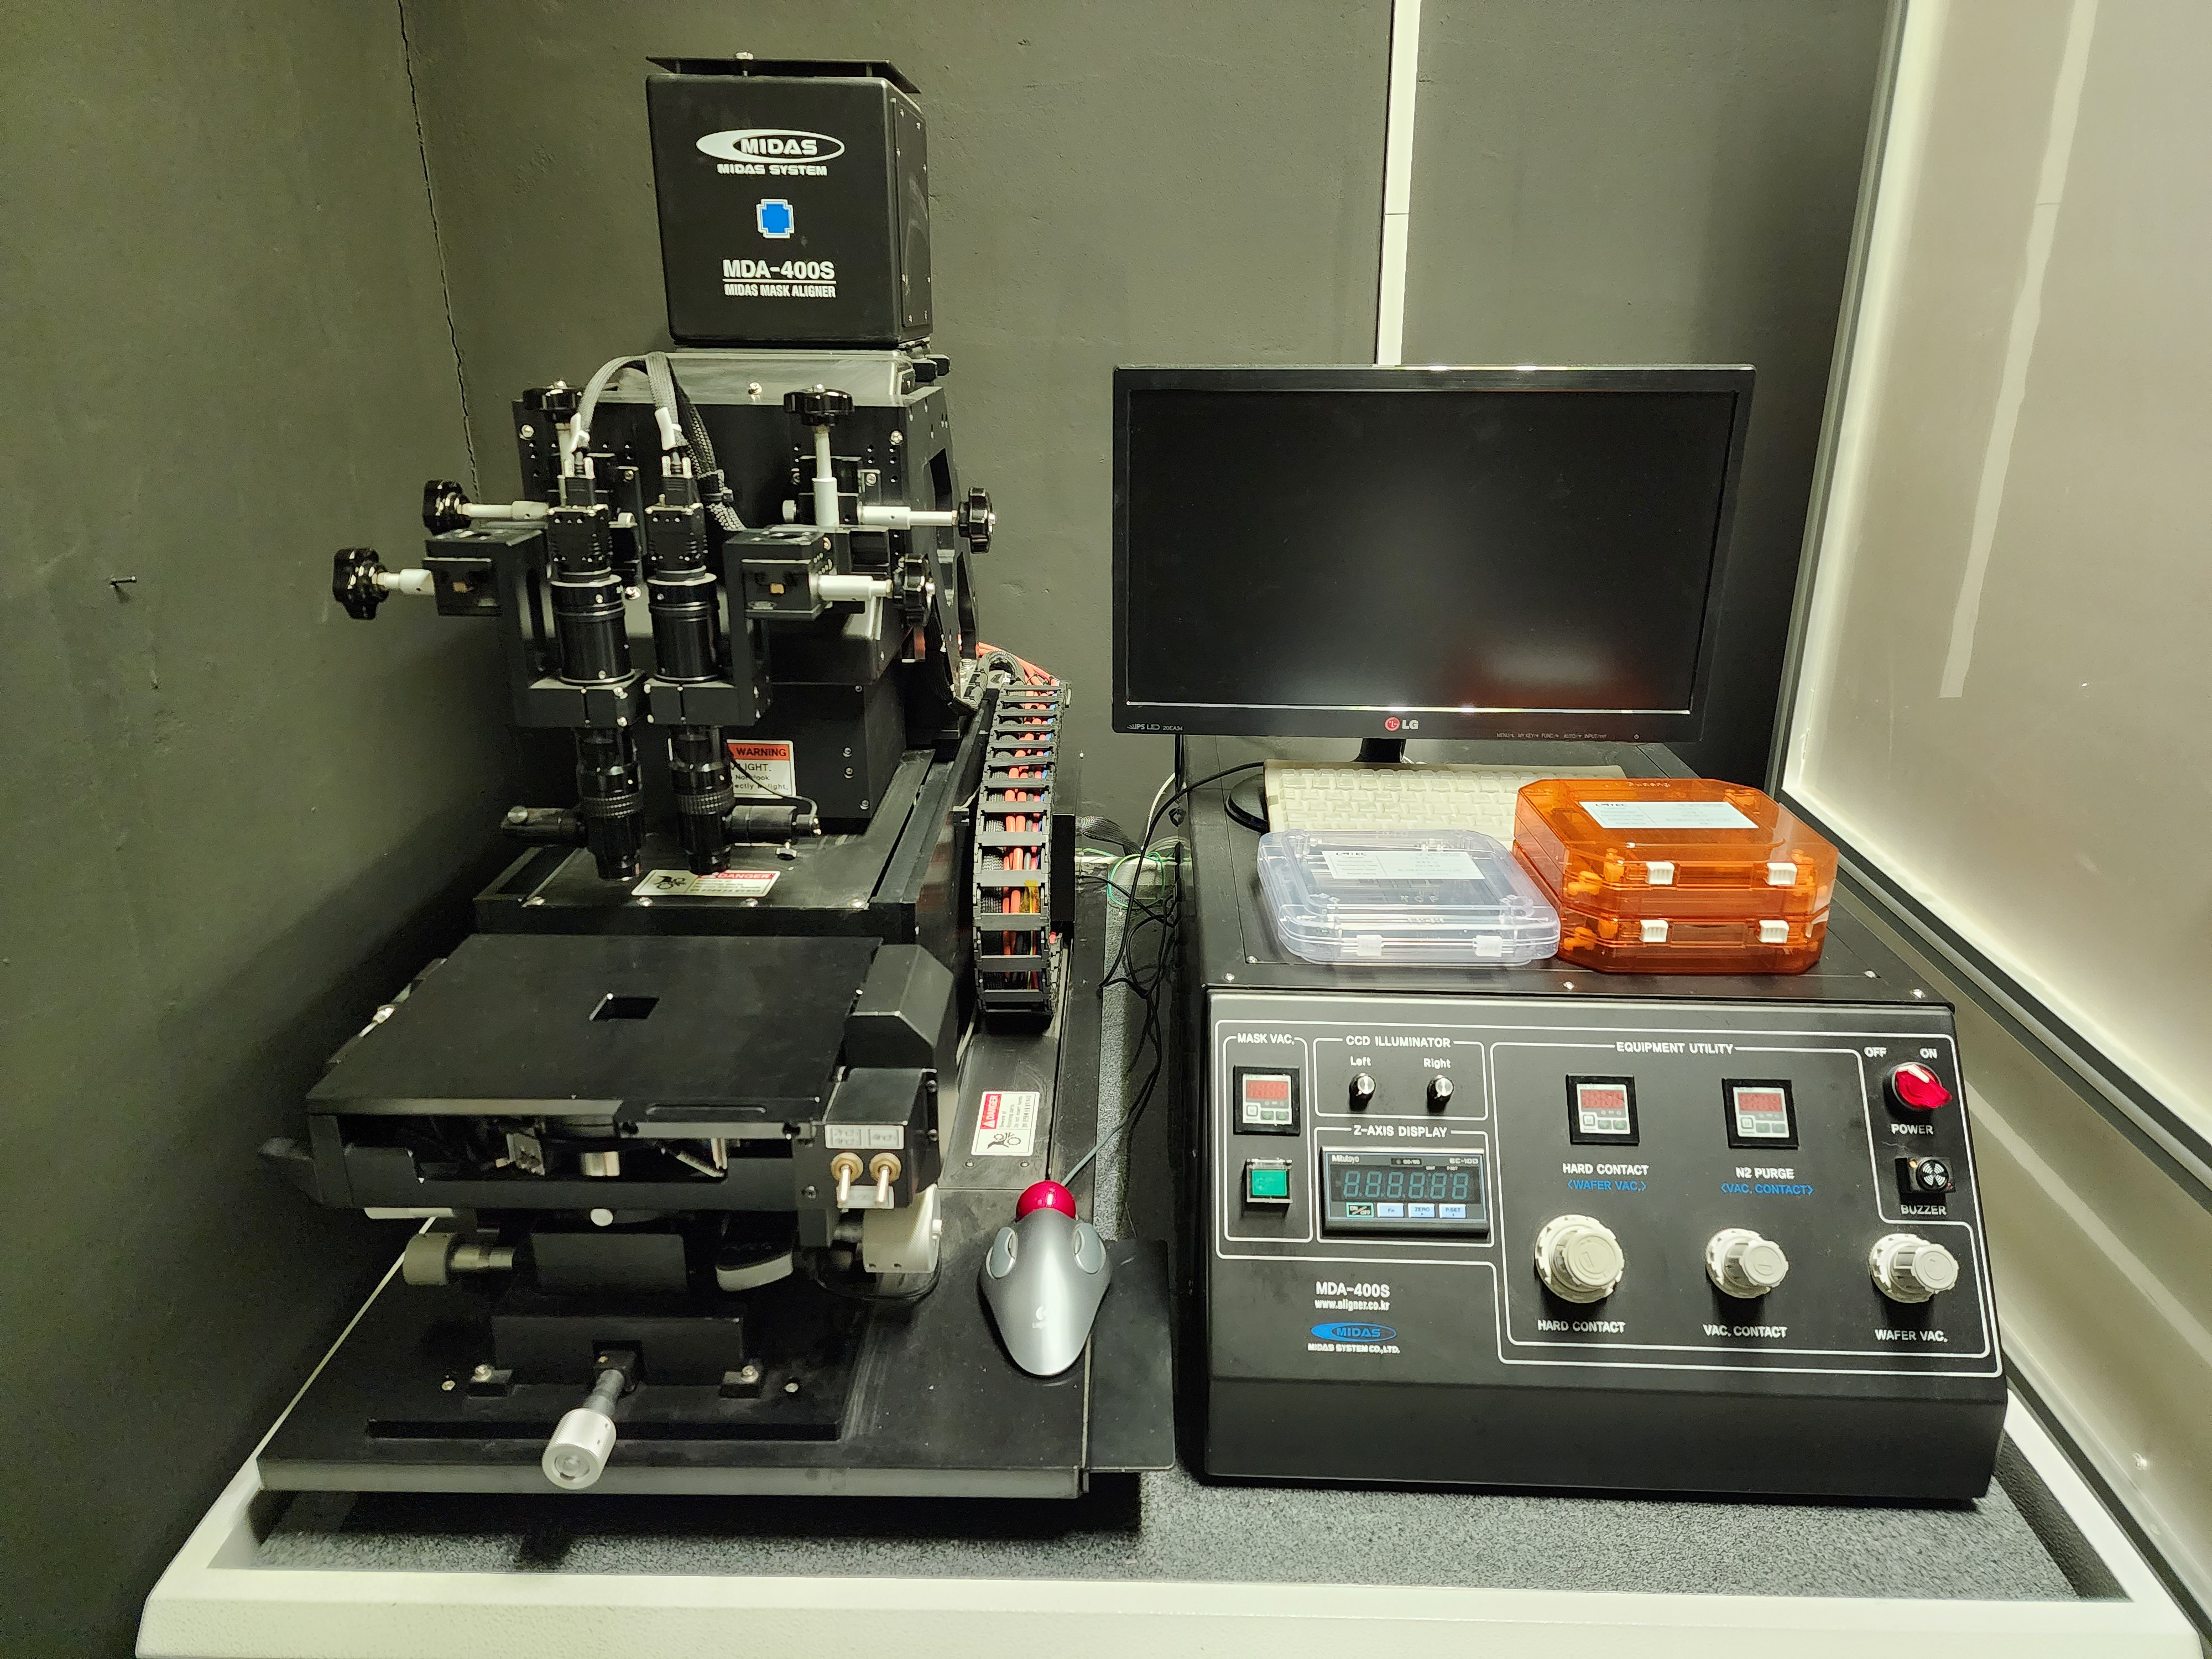
\includegraphics[scale=0.04]{violet.JPG}
    \caption{Exposure에 사용한 기기.}
    \label{fig:violet}
  \end{figure}
  기기를 열고 mask(FIG.~\ref{fig:mask})를 부착한 다음, 기판을 올려놓고 기기를 닫는다.
  Mask와 기판은 기기가 진공을 이용해 고정한다. 자외선을 노출시키는 동안
  실험자의 건강에 유의하여 기기를 직접 바라보지 않도록 한다.
  \begin{figure}[htbp]
    \centering
    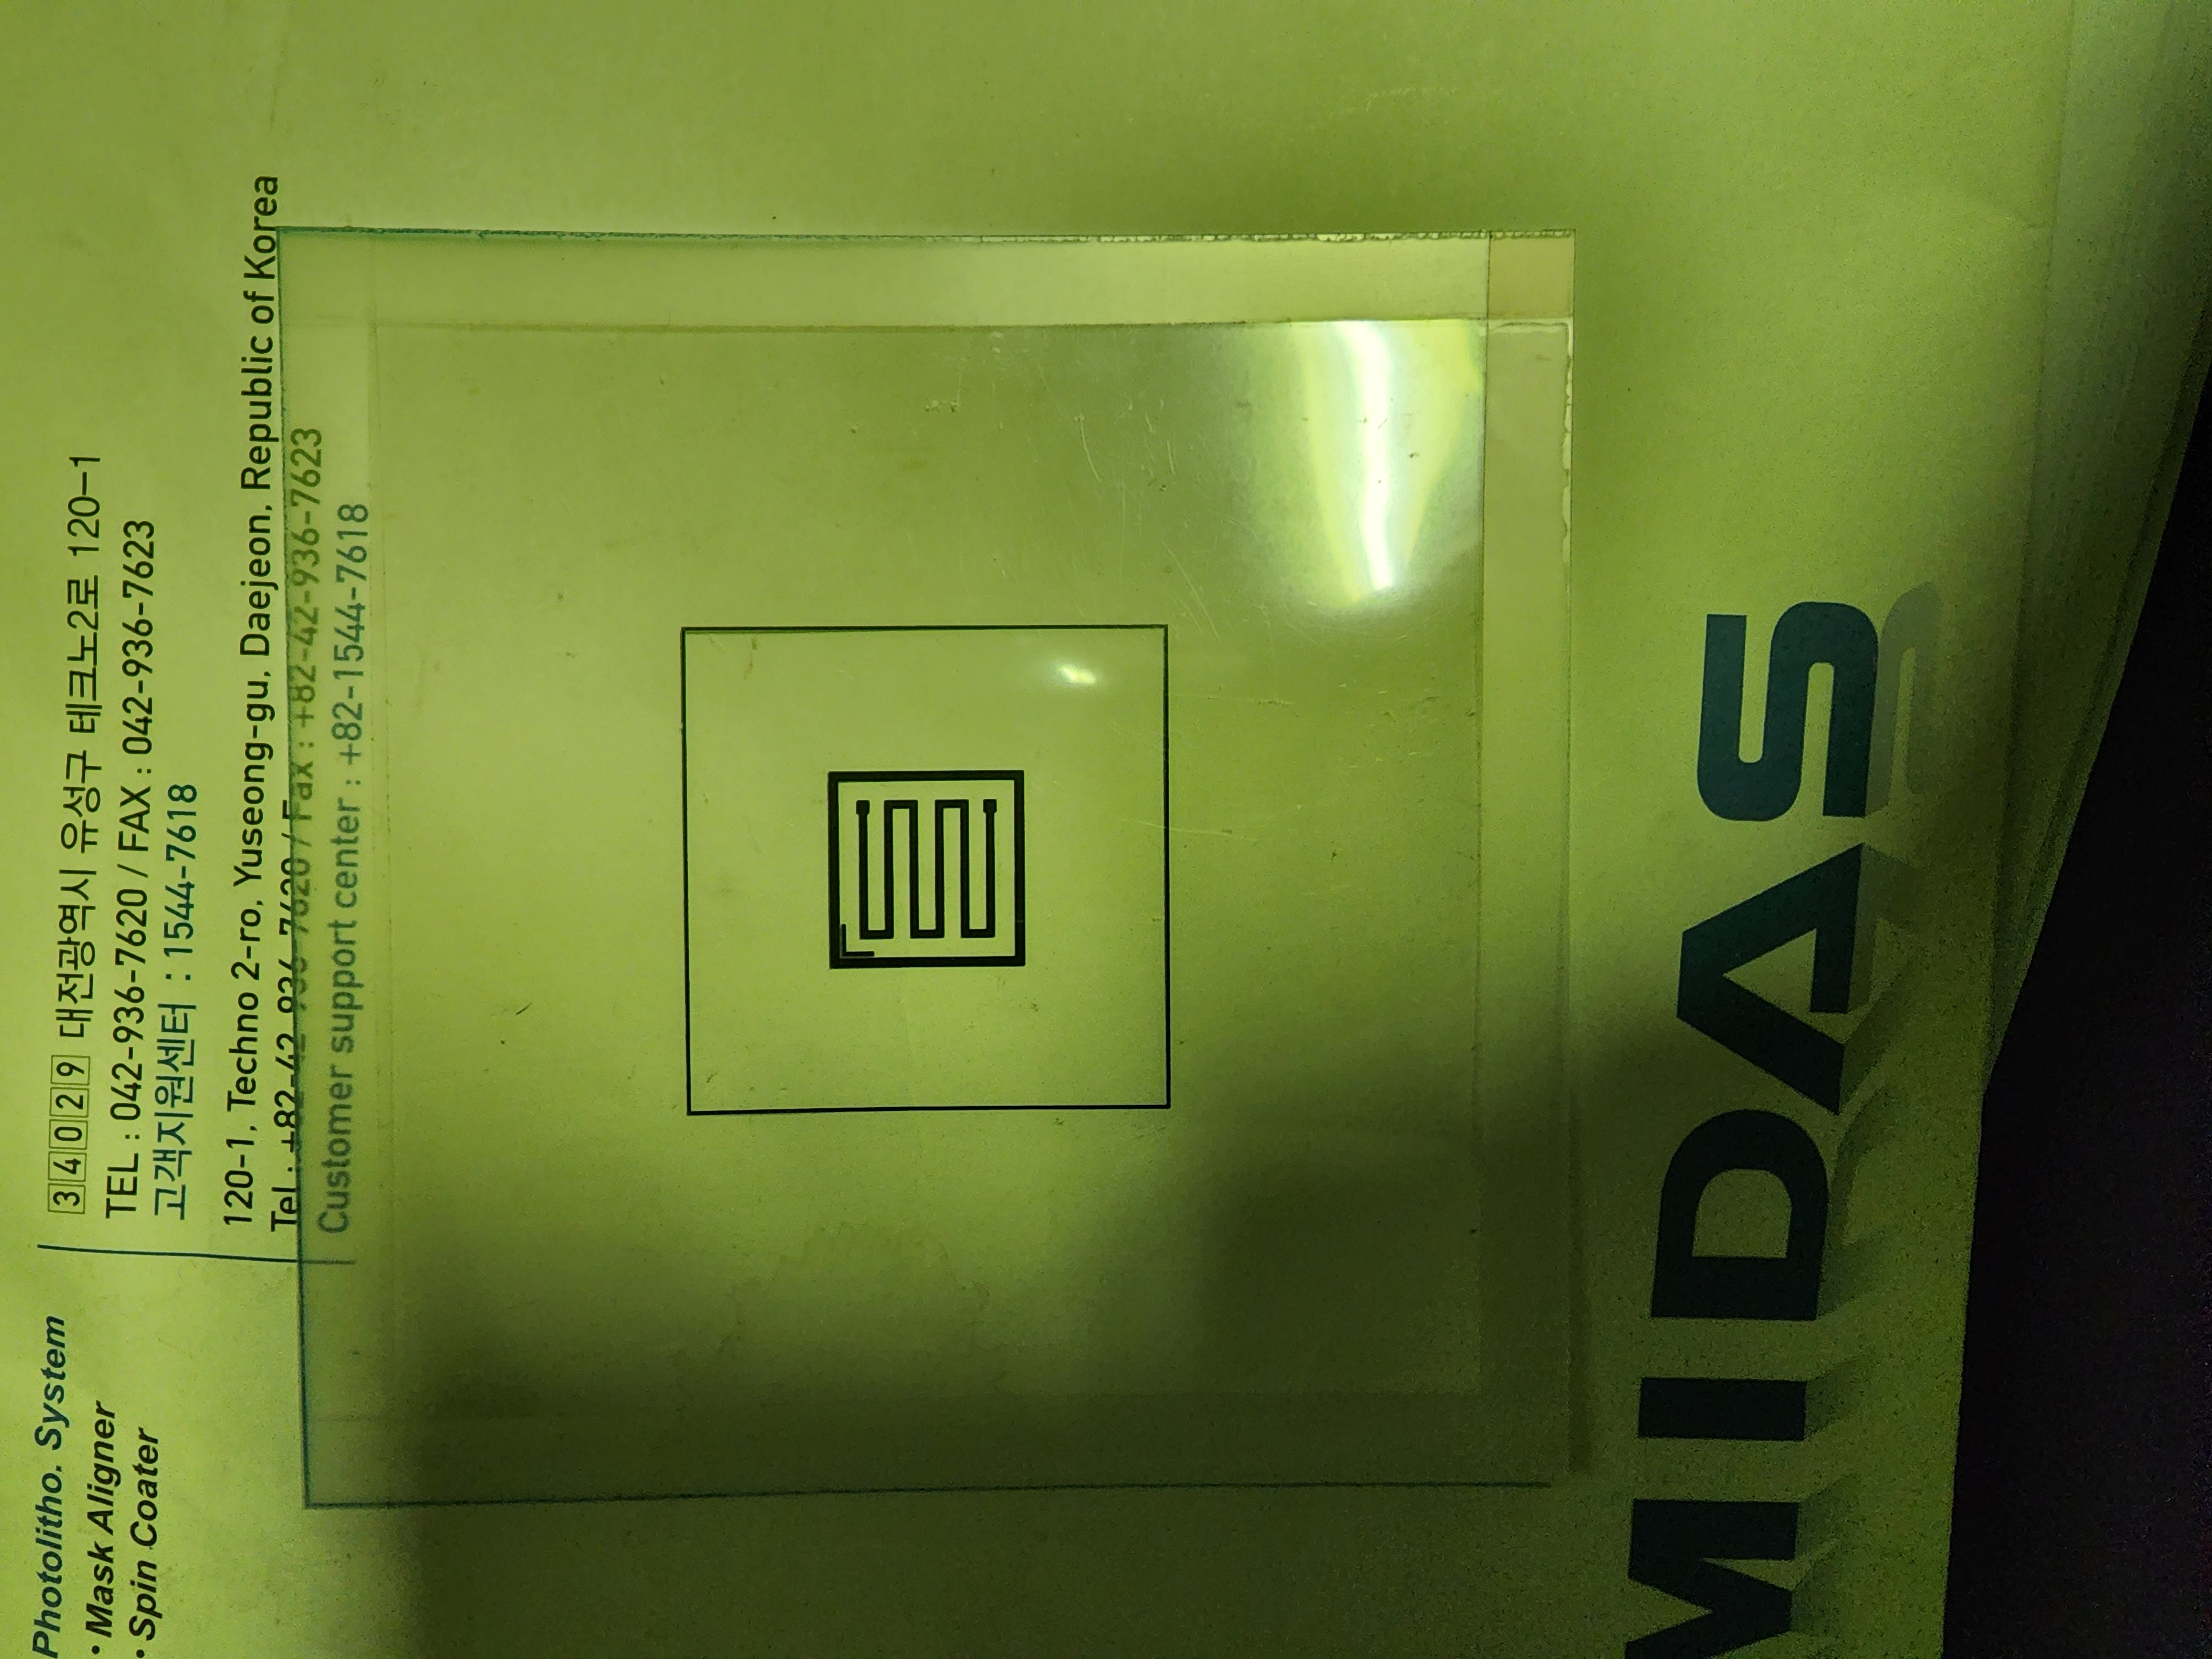
\includegraphics[scale=0.04]{mask.JPG}
    \caption{Exposure에 사용한 mask.}
    \label{fig:mask}
  \end{figure}

  \item[5. ] 기판을 현상액에 노출시켜 감광물질을 제거한다.
  감광물질 제거 후 현상액이 남아있을 수 있어 증류수로 기판을 세척한다.
  세척 후 블로워를 이용해 기판에 남아있는 증류수를 제거한다.

  \item[6. ] Exposure가 완료된 기판을 한번 더 가열한다.
  각 기판을 110~$^\circ$C의 온도에 90초 간 가열하였다.

  \item[7. ] 기판에 금속을 증착한다(FIG.~\ref{fig:jc}). 

  \begin{figure}[htbp]
    \centering
    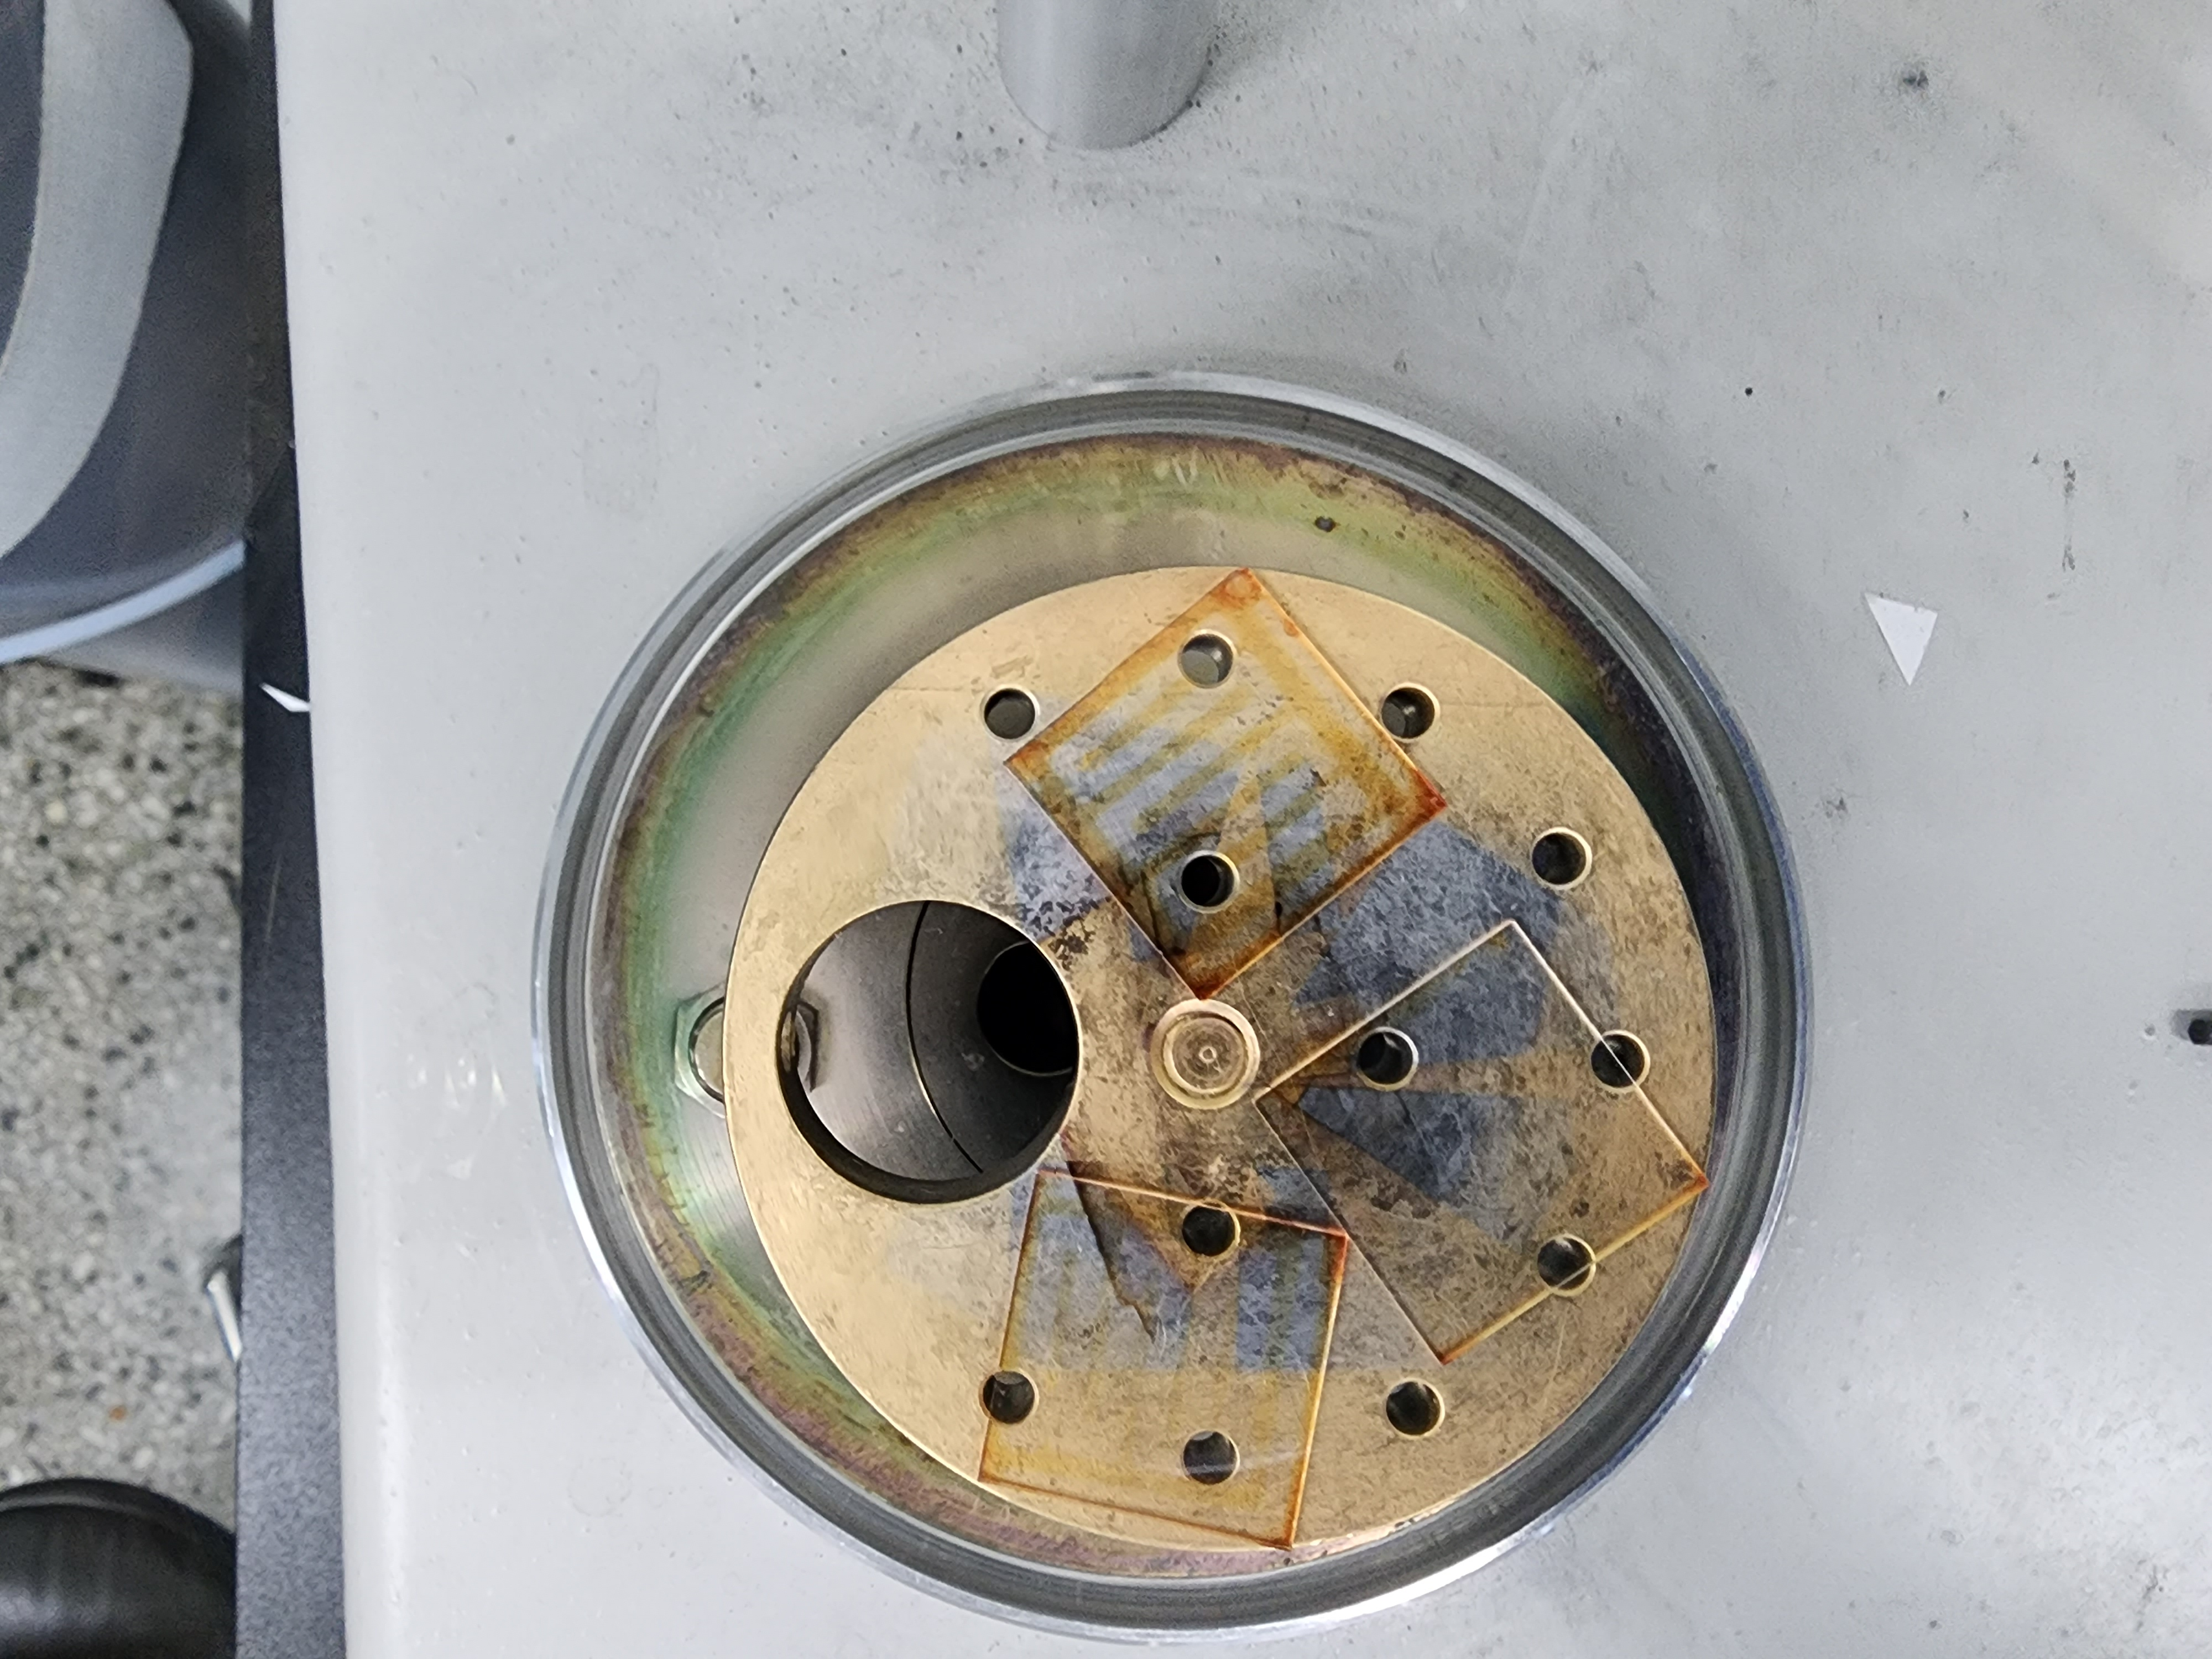
\includegraphics[scale=0.04, angle=270]{before.JPG}
    \caption{증착 전 기판의 모습.}
    \label{fig:before}
  \end{figure}
  기기 안에 기판을 넣고 작동시키면 기기가 진공을 만든 상태에서 240초 간 
  기판의 표면에 금속을 증착한다(FIG.~\ref{fig:after}).
  
  \begin{figure}[htbp]
    \centering
    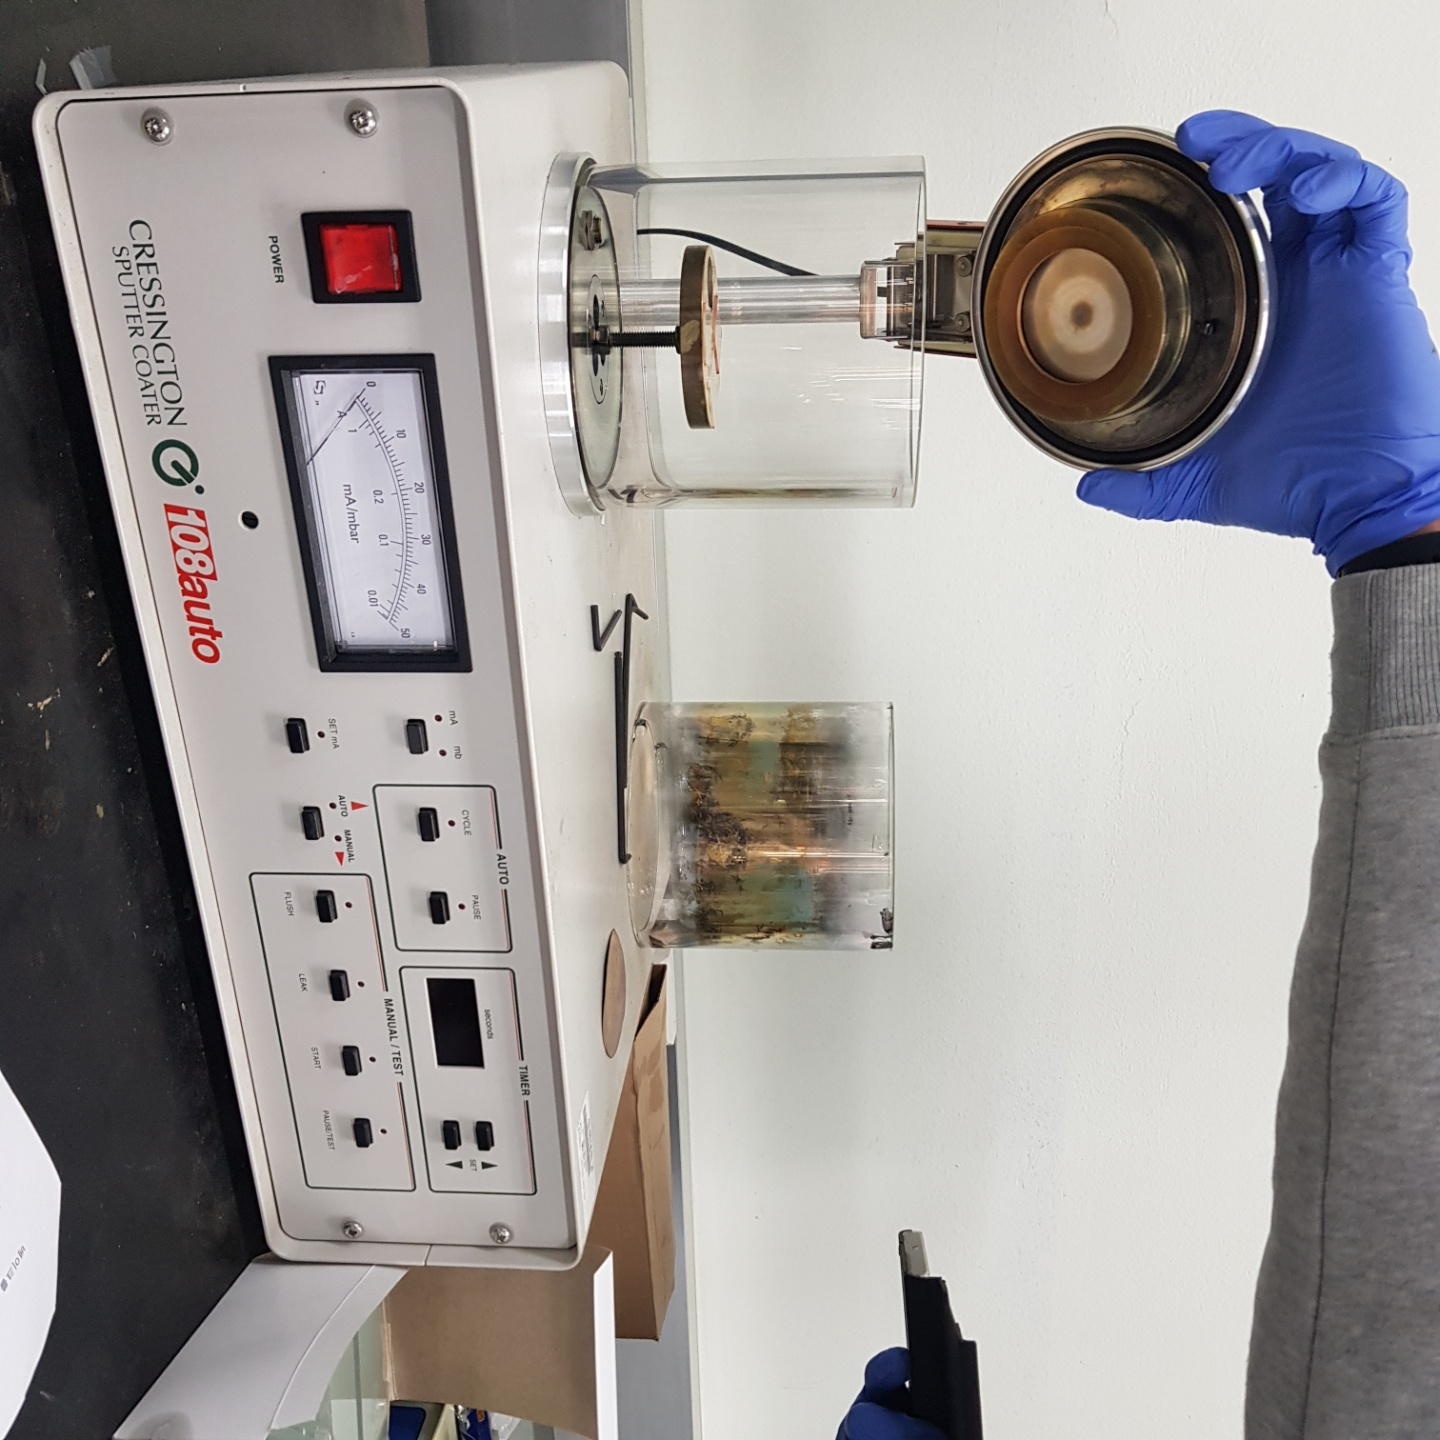
\includegraphics[scale=0.1, angle=90]{jc.JPG}
    \caption{증착에 사용한 기기.}
    \label{fig:jc}

    \centering
    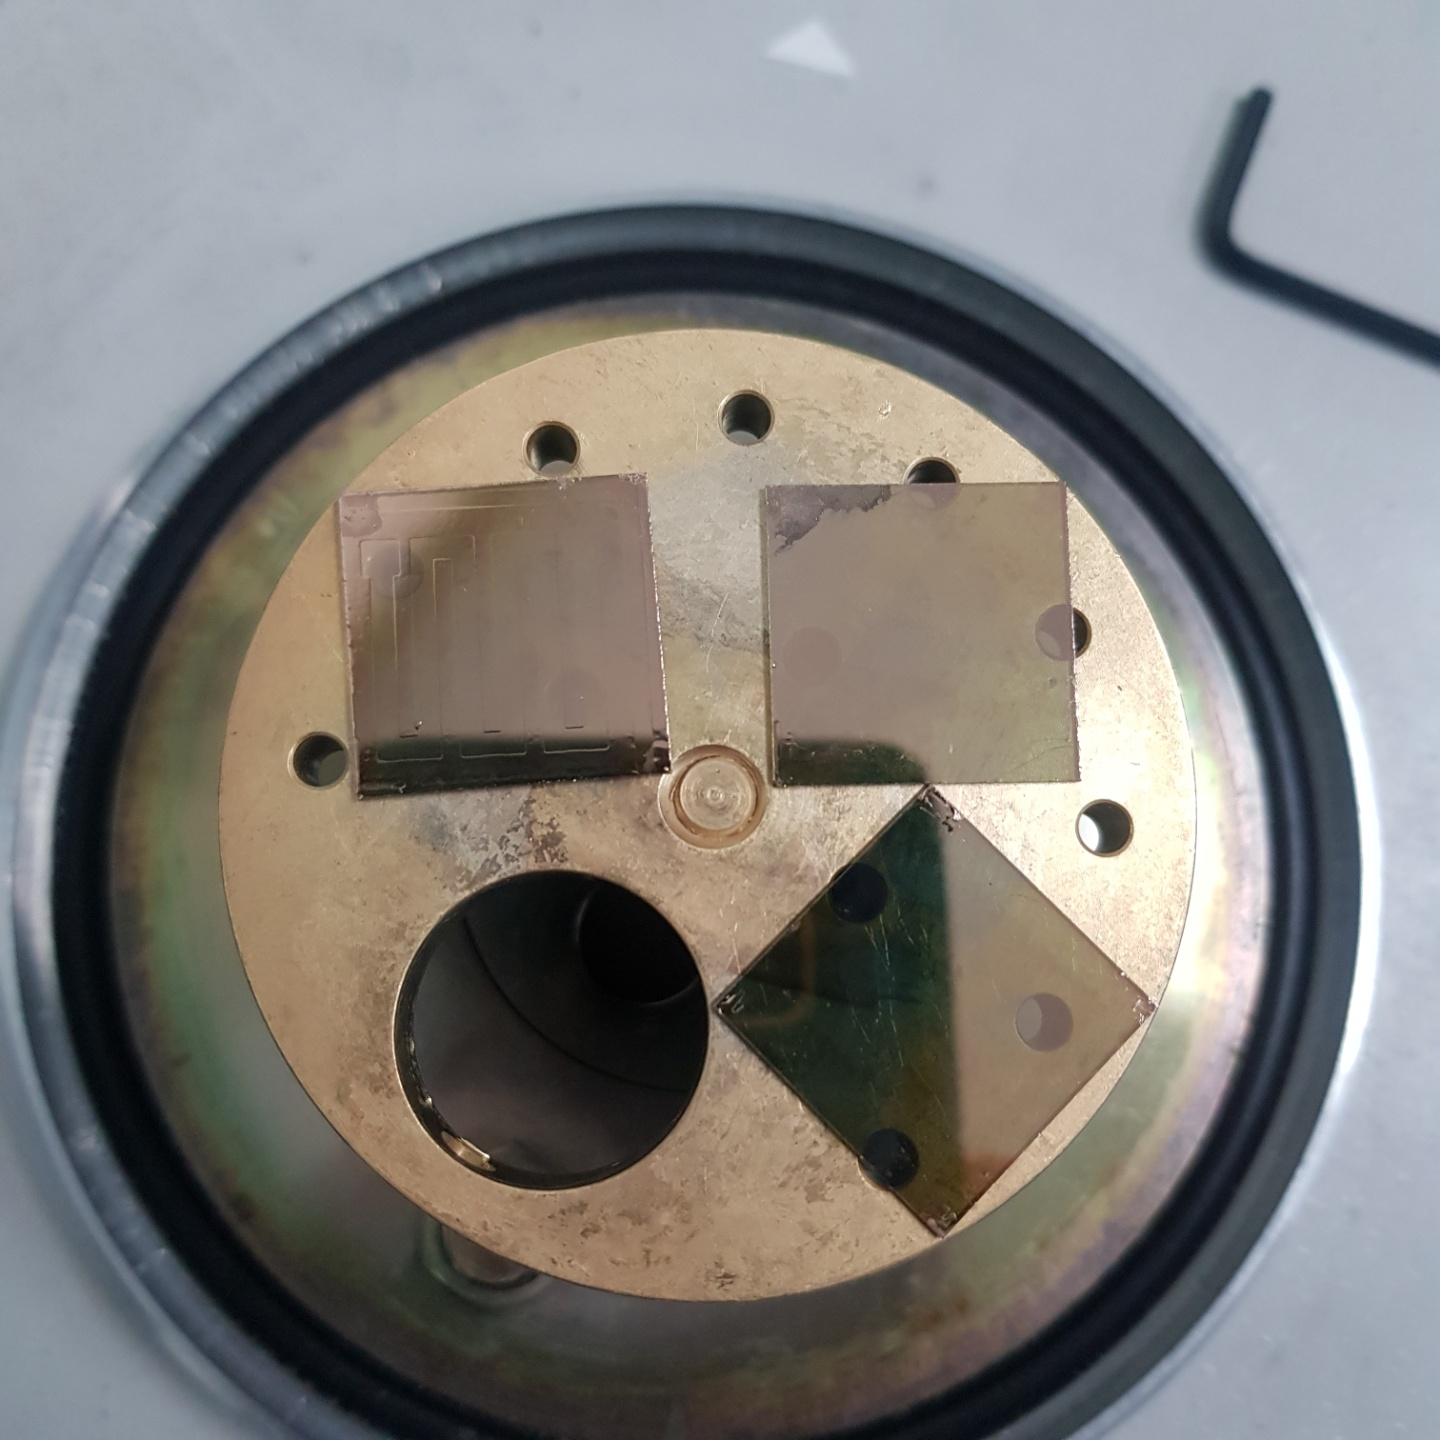
\includegraphics[scale=0.1]{after.JPG}
    \caption{증착이 완료된 기판의 모습.}
    \label{fig:after}
  \end{figure}



  \item[8. ] 증착이 완료된 기판의 표면에서 감광물질을 제거한다. 감광물질을 제거하면
  감광물질 위에 쌓였던 금속도 같이 제거되며 기판의 표면에 직접 증착된 금속만 
  남게된다(FIG.~\ref{fig:result}).
  본 실험에서는 초음파 세척기를 이용해 감광물질을 제거하였다.
  \begin{figure}[htbp]
    \centering
    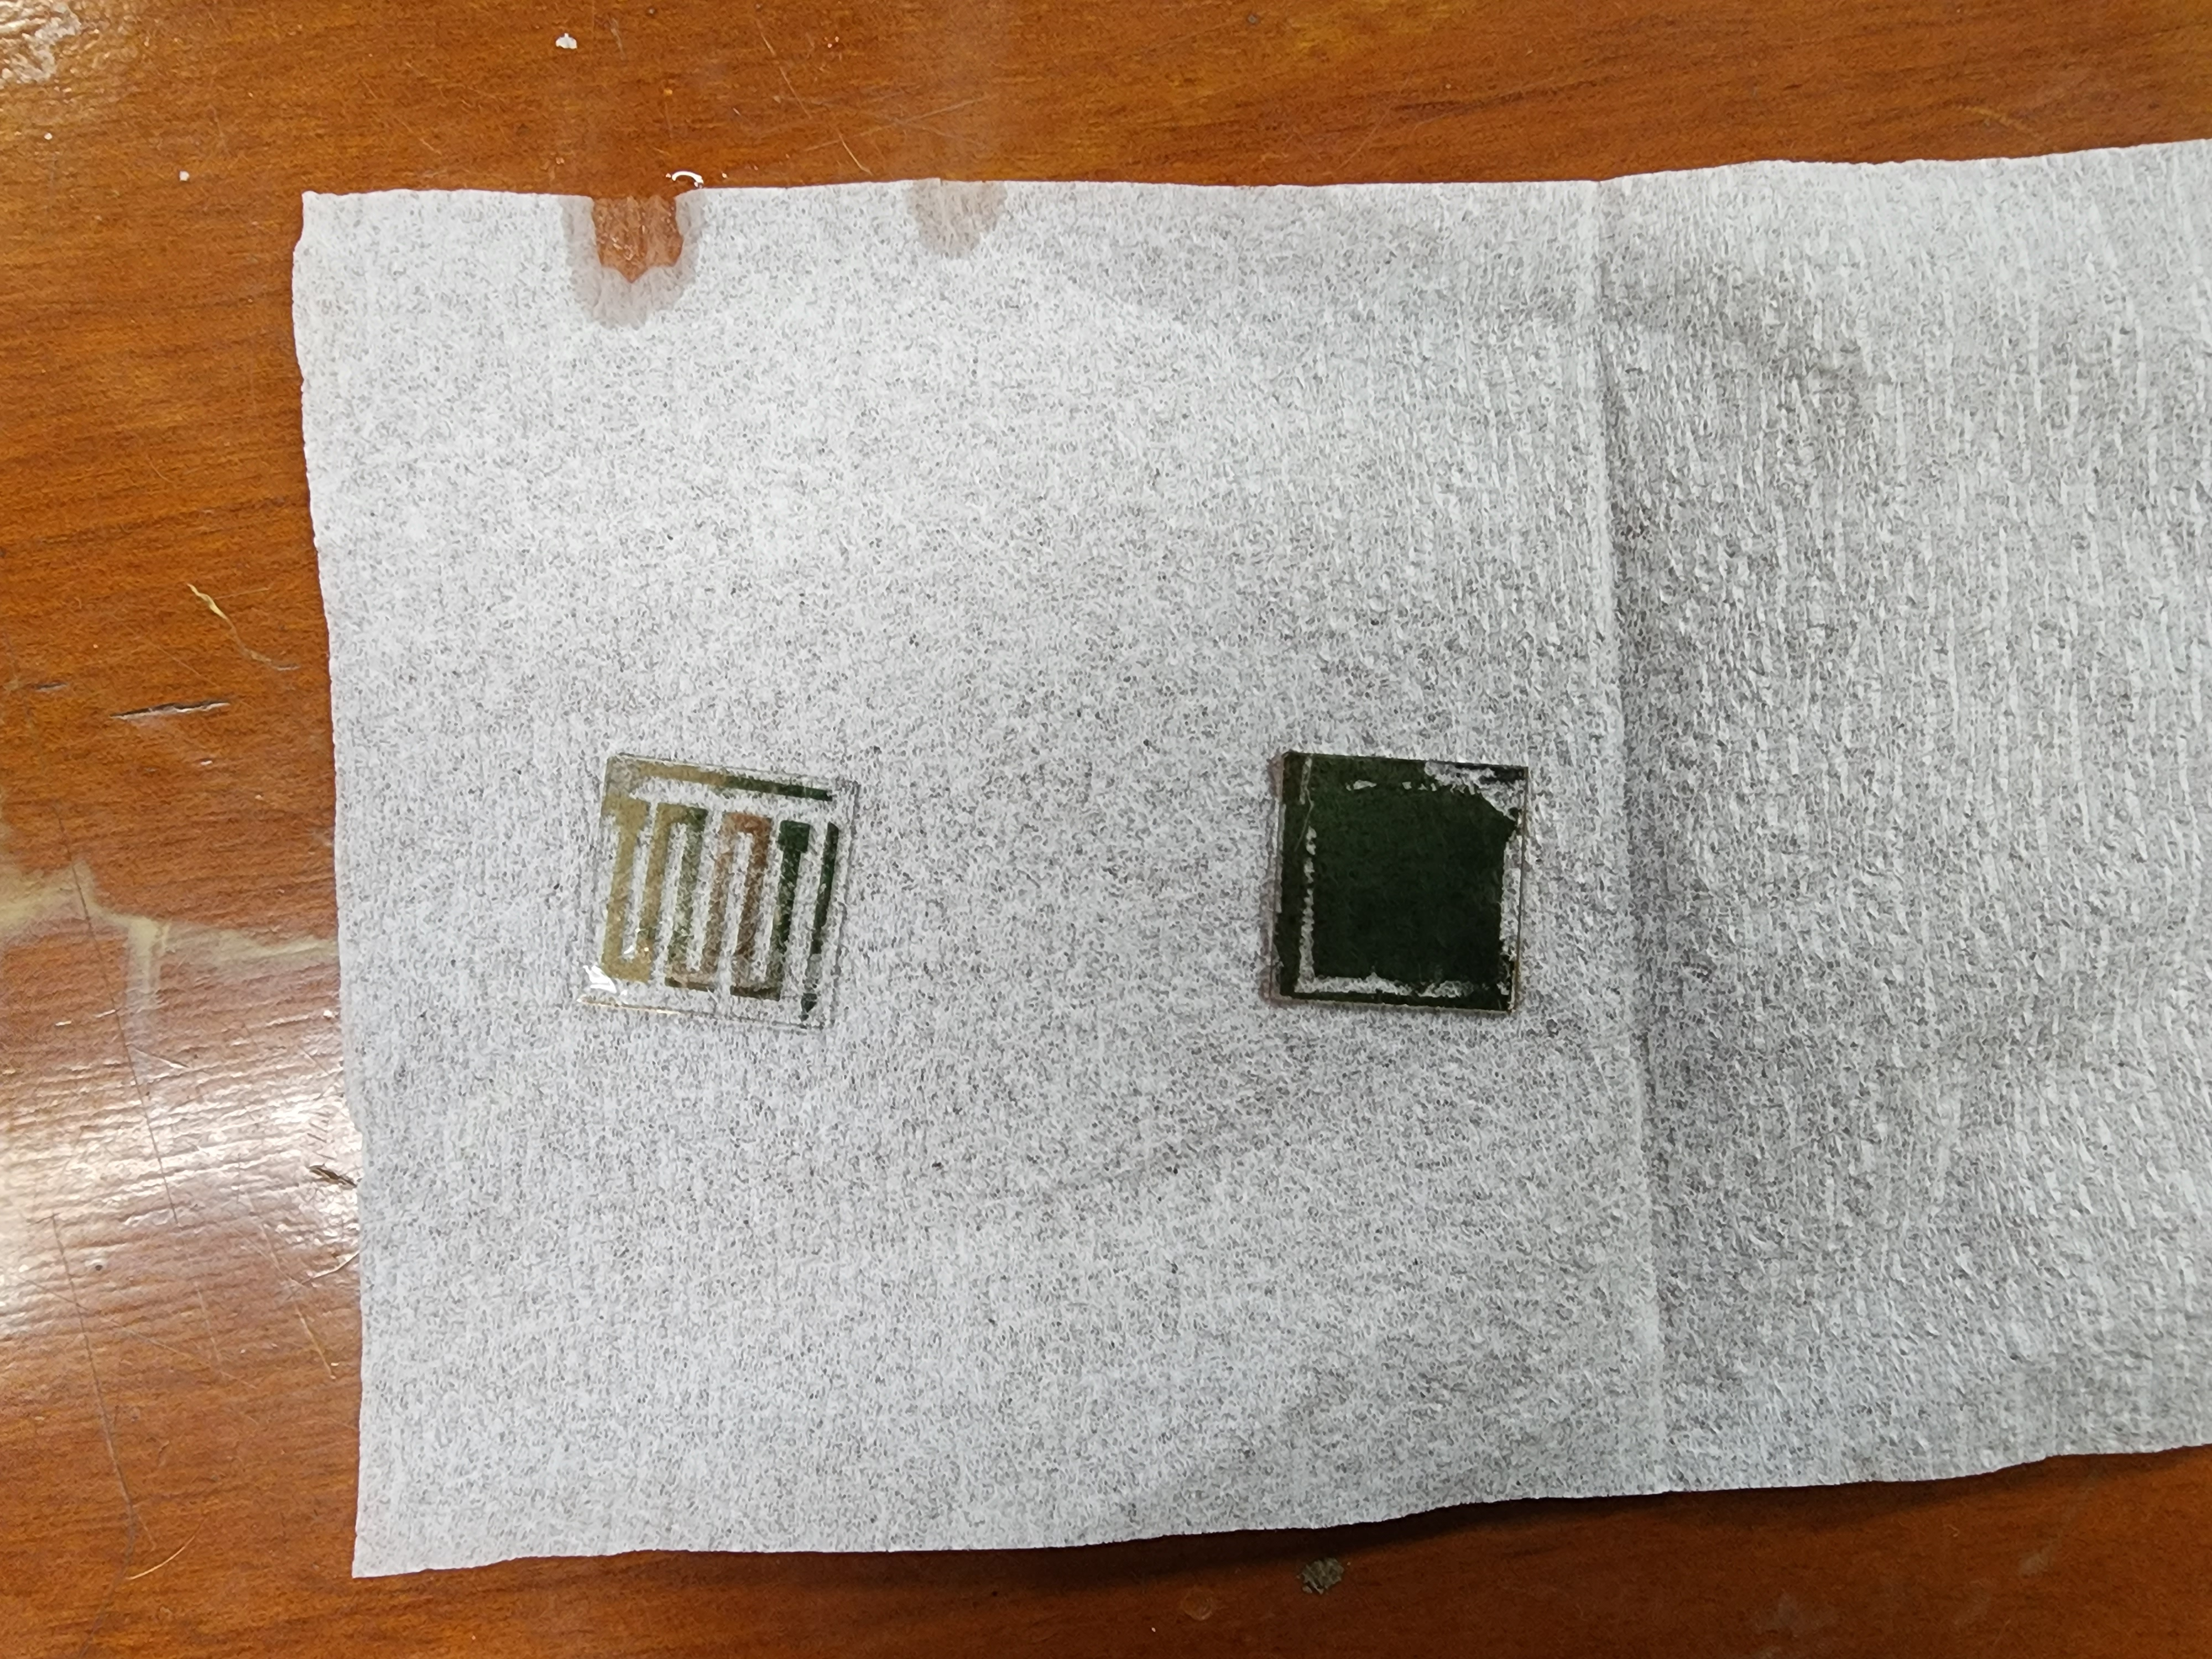
\includegraphics[scale=0.05, angle=0]{result.JPG}
    \caption{감광물질을 제거한 기판의 모습.}
    \label{fig:result}
  \end{figure}
\end{itemize}

\newpage
\section{Result}
총 네개의 기판 중, 4000 RPM의 조건에서 사용한 기판의 크기가 너무 커 감광물질 도포 단계에서
기기가 기판을 충분히 고정할 수 없어 세개의 기판을 가지고 실험을 진행하였다.
\subsubsection{1000 RPM}
  1000 RPM으로 감광물질을 도포한 기판에서는 mask의 pattern이 선명하게 나타났다. 
\subsubsection{2000 RPM}
  2000 RPM으로 감광물질을 도포한 기판에서는 mask의 pattern이 나타나지 않았으며
  기판의 모든 표면에 금속이 증착되었다. 
\subsubsection{3000 RPM}
  1000 RPM으로 감광물질을 도포한 기판에서는 mask의 pattern이 선명하게 나타나지 않았으며
  테두리 부분의 pattern 이 일부분 나타났다. 
\subsection{Conclusion}
\begin{itemize}
  \item[1. ] 1000 RPM의 조건에서 사용한 기판에 나타난 pattern은 mask가 자외선을 차단한
  부분이었다. 이는 mask가 자외선을 차단한 부분에서 기판의 표면에 금속이 직접 증착되었을을
  의미하며, 이를 통해 현상액에 제거된 감광물질은 자외선이 조사되지 않은 감광물질임을
  알 수 있다. 따라서 이번 실험에 사용된 감광물질이 negative임을 추정할 수 있다.



  \item[2. ] FIG.~\ref{fig:result}에서 모든 과정을 마친 기판의 갯수가 2개 뿐인데
  2000 RPM의 조건에서 사용한 기판은 과정 중에 떨어트려 감광물질을 도포한 표면이
  어느쪽인지 판단할 수 없었다. 금속을 증착시킬 때 감광물질이 도포된 표면을 위로 향하게
  했어야 하는데 도포되지 않은 표면이 위로 향하여 표면의 모든 부분에 금속이 직접 증착되어
  pattern이 나타나지 않았다. 증착 전에 약간의 pattern이 보였던 것으로 보아, 표면을
  올바르게 향하여 금속을 증착하였다면 1000 RPM의 조건에서 사용한 기판만큼 선명한 결과를
  얻을 수 있었을 것으로 생각된다.



  \item[3. ] 3000 RPM의 조건에서 사용한 기판에 나타난 pattern은 가장자리에서
  mask의 pattern과 유사하게 나타났고 가운데 부분에서는 감광물질이 벗겨지지 않았다.
  그 이유로 스핀 코팅과정에서 기판을 더욱 빠르게 회전시킬 수록 감광물질이 얇게 도포되어
  감광물질이 너무 얇게 증착된 것을 생각해볼 수 있다. 이로 인해 현상액이 감광물질을 제거할 때
  감광물질이 충분한 두께를 가지지 못했다면 증착된 금속이 제거되지 않을 수도 있다.
  

  
  
  

\end{itemize}

\nocite{*} 
\bibliography{ref}



%\begin{thebibliography}{9}
%\end{thebibliography}

\vfill
\end{document}